\documentclass[12pt,letterpaper]{exam}
\usepackage[lmargin=1in,rmargin=1in,tmargin=1in,bmargin=1in]{geometry}
\usepackage{../style/exams}

% -------------------
% Course & Exam Information
% -------------------
\newcommand{\course}{MATH 122: Exam 2}
\newcommand{\term}{Fall --- 2024}
\newcommand{\examdate}{10/15/2024}
\newcommand{\timelimit}{75 Minutes}

\setbool{hideans}{true} % Student: True; Instructor: False

% -------------------
% Content
% -------------------
\begin{document}

\examtitle
\instructions{Write your name on the appropriate line on the exam cover sheet. This exam contains \numpages\ pages (including this cover page) and \numquestions\ questions. Check that you have every page of the exam. Answer the questions in the spaces provided on the question sheets. Be sure to answer every part of each question and show all your work. If you run out of room for an answer, continue on the back of the page --- being sure to indicate the problem number.} 
\scores
\bottomline
\newpage


% -------------------
% Questions
% -------------------
\begin{questions}

% Question 1
\newpage
\question[20] Consider the function $f(x)$ plotted below. 
	\[
	\fbox{
	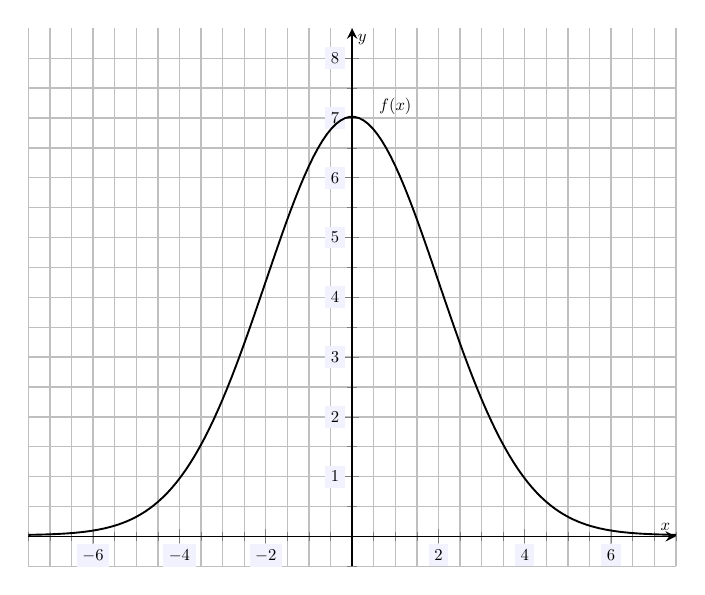
\begin{tikzpicture}[scale=1.2,every node/.style={scale=0.5}]
	\begin{axis}[
	grid=both,
	axis lines=middle,
	ticklabel style={fill=blue!5!white},
	xmin= -7.5, xmax=7.5,
	ymin= -0.5, ymax=8.5,
	xtick={-8,-6,...,8},
	ytick={-1,0,...,8},
	minor tick = {-8,-7.5,...,8},
	xlabel=\(x\),ylabel=\(y\),
	]
	\addplot[line width= 0.02cm,samples=200,domain= -10.5:10.5] ({x},{7*e^(-x^2/8) + 0.02});
	\node at (1,7.2) {$f(x)$};
	\end{axis}
	\end{tikzpicture}
	}
	\] \par
Based on the plot above, answer the following: \par
	\begin{enumerate}[(a)]
        	\item On what interval(s)---if any---is $f'(x) > 0$? \vfill
	\item On what interval(s)---if any---is $f'(x) < 0$? \vfill
	\item Find any points of inflection---if any. \vfill
	\item On what interval(s)---if any---is $f''(x) > 0$? \vfill
	\item On what interval(s)---if any---is $f''(x) < 0$? \vfill
	\item Determine whether the following are positive ($> 0$), negative ($< 0$), or zero ($= 0$): \pvspace{0.1cm} 
		\begin{2itemize}
		\item $f(-2)$ \hspace{0.1cm} \underline{\phantom{==$\approx$==}} \hspace{0.1cm} 0 
		\item $f'(0)$ \phantom{$-$} \underline{\phantom{==$\approx$==}} \hspace{0.1cm} 0
		\item $f''(5)$ \phantom{$'''$} \underline{\phantom{==$\approx$==}} \hspace{0.1cm} 0
		\item $f'(-3)$ \underline{\phantom{==$\approx$==}} \hspace{0.1cm} 0 \pvspace{0.2cm}
		\item $f'(5)$ \phantom{$.'$} \underline{\phantom{==$\approx$'....''}} \hspace{0.1cm} 0 \pvspace{0.2cm}
		\item $f''(0)$ \phantom{$l$} \underline{\phantom{==$\approx$'....''}} \hspace{0.1cm} 0
		\end{2itemize} 
	\item Sketch the tangent line to $f(x)$ at $x= 4$ on the graph above. 
	\end{enumerate}



% Question 2
\newpage
\question[15] Showing all your work, compute the derivatives given below. {\itshape Do not simplify your answer.} \pvspace{0.3cm}
	\begin{enumerate}[(a)]
	\item $\dfrac{d}{dx} \left( x^6 - 3x + \dfrac{1}{\sqrt{x}} - 11 \right)=$ \vfill
	\item $\dfrac{d}{dx} (x^{10}\, 2^x)=$ \vfill
	\item $\dfrac{d}{dx}\, \ln(5x^2 - x)=$ \vfill
	\item $\dfrac{d}{dx} \, (5\pi^3)=$ \vfill
	\item $\dfrac{d}{dx} \left(\dfrac{6x - 1}{x^2 + 1} \right)=$ \vfill
	\end{enumerate}



% Question 3
\newpage
\question[15] Consider the \textit{derivative} of a function, $f'(x)$, plotted below. 
	\[
	\fbox{
	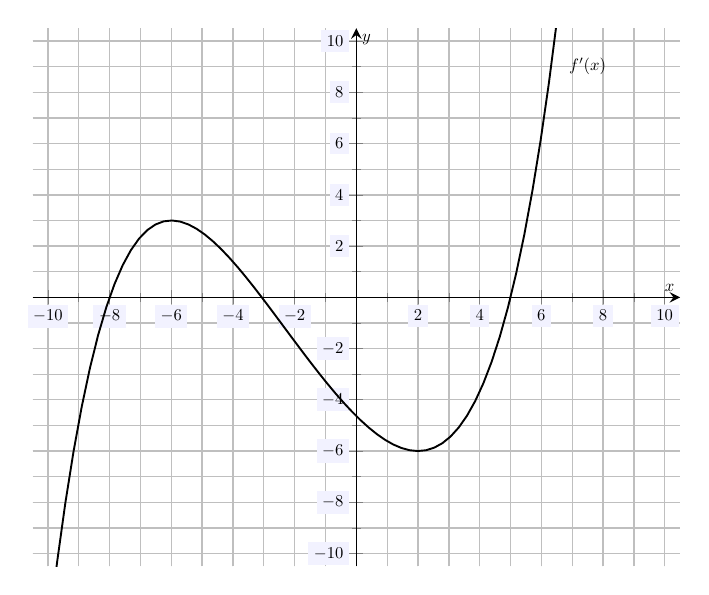
\begin{tikzpicture}[scale=1.2,every node/.style={scale=0.5}]
	\begin{axis}[
	grid=both,
	axis lines=middle,
	ticklabel style={fill=blue!5!white},
	xmin= -10.5, xmax=10.5,
	ymin= -10.5, ymax=10.5,
	xtick={-10,-8,-6,-4,-2,0,2,4,6,8,10},
	ytick={-10,-8,-6,-4,-2,0,2,4,6,8,10},
	minor tick = {-10,-9,...,10},
	xlabel=\(x\),ylabel=\(y\),
	]
	\addplot[line width= 0.02cm,samples=80,domain= -10.5:10.5] ({x},{-4.6345 - 1.19714*x + 0.18566*x^2 + 0.030597*x^3 + 0.0020121*x^4 + 0.000286889*x^5});
	\node at (7.5,9) {$f'(x)$};
	\end{axis}
	\end{tikzpicture}
	}
	\] 
Based on the plot above, answer the following questions: 
	\begin{enumerate}[(a)]
	\item On what interval(s)---if any---is $f(x)$ increasing? \vfill
	\item On what interval(s)---if any---is $f(x)$ decreasing? \vfill
	\item On what interval(s)---if any---is $f(x)$ concave up? \vfill
	\item On what interval(s)---if any---is $f(x)$ concave down? \vfill
	\item Find any critical values for $f(x)$---if any. \vfill
	\item Classify any critical values you found in (e). \vfill
	\item Find any points of inflection for $f(x)$. \vfill
	\end{enumerate}



% Question 4
\newpage
\question[15] Showing all your work, compute the derivatives given below. {\itshape Do not simplify your answer.} \pvspace{0.3cm}
	\begin{enumerate}[(a)]
	\item $\dfrac{d}{dx} (3x^2\, e^{-x}\, \log_5(x) \big)=$ \vfill
	\item $\dfrac{d}{dx} \big(9^{x^3} - x \big)^7=$ \vfill
	\item $\dfrac{d}{dx} \left( \dfrac{(3x - 1) e^{2x}}{\ln(1 - x)} \right)=$ \vfill
	\end{enumerate}



% Question 5
\newpage
\question[15] A company produces widgets. They hire financial analysts to examine their production costs. The analysts determine that if $q$ items are produced, then the total production cost for the widgets is given by $C(q)= 223,\!000 + 1,\!000q - q^2$. 
	\begin{enumerate}[(a)]
	\item Find the fixed costs for producing these widgets. 
	\item Find the marginal costs at a production level of $q= 180$.
	\item What level of production maximizes the total cost of producing these widgets? Be sure to justify your answer with either the first or second derivative test. 
	\end{enumerate}



% Question 6
\newpage
\question[5] Consider the graphs of the functions $f(x)$ and $g(x)$ given below.
	\[
	\fbox{
	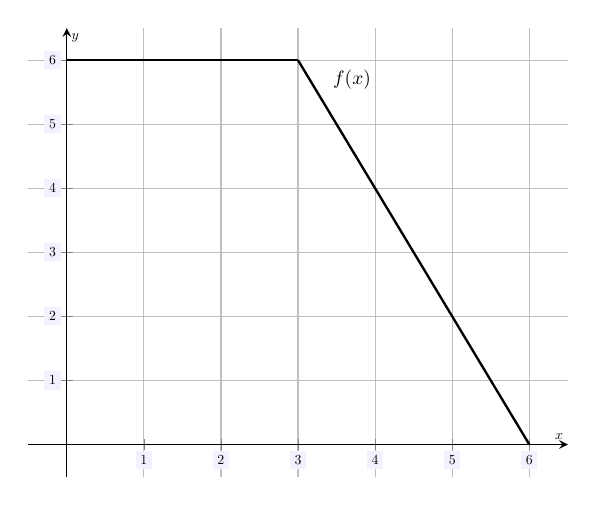
\begin{tikzpicture}[scale=1,every node/.style={scale=0.5}]
	\begin{axis}[
	grid=both,
	axis lines=middle,
	ticklabel style={fill=blue!5!white},
	xmin= -0.5, xmax=6.5,
	ymin= -0.5, ymax=6.5,
	xtick={-1,0,...,6},
	ytick={-1,0,...,6},
	minor tick = {-1,0,...,6},
	xlabel=\(x\),ylabel=\(y\),
	]
	\addplot[line width= 0.03cm,samples=10,domain= 0:3] ({x},{6});
	\addplot[line width= 0.03cm,samples=10,domain= 3:6] ({x},{2*(6 - x)});
	\node at (3.7,5.7) {\scalebox{1.4}{$f(x)$}};
	\end{axis}
	\end{tikzpicture}
	} \hspace{0.5cm}
	\fbox{
	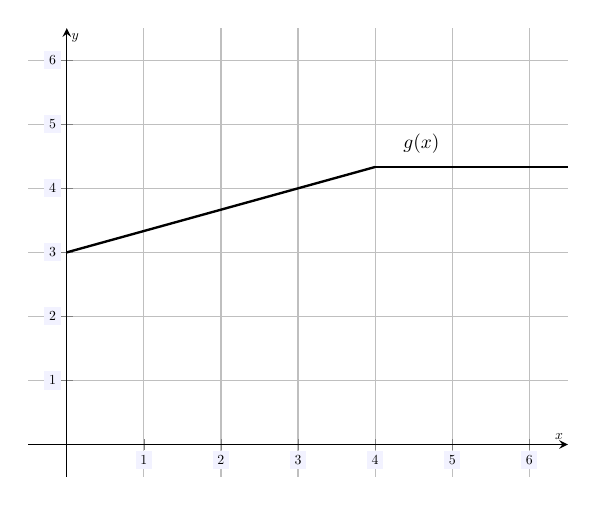
\begin{tikzpicture}[scale=1,every node/.style={scale=0.5}]
	\begin{axis}[
	grid=both,
	axis lines=middle,
	ticklabel style={fill=blue!5!white},
	xmin= -0.5, xmax=6.5,
	ymin= -0.5, ymax=6.5,
	xtick={-1,0,...,6},
	ytick={-1,0,...,6},
	minor tick = {-1,0,...,6},
	xlabel=\(x\),ylabel=\(y\),
	]
	\addplot[line width= 0.03cm,samples=10,domain= 0:4] ({x},{1/3*x + 3});
	\addplot[line width= 0.03cm,samples=10,domain= 4:6.5] ({x},{13/3});
	\node at (4.6,4.7) {\scalebox{1.4}{$g(x)$}};
	\end{axis}
	\end{tikzpicture}
	}
	\]
Based on these plot and showing all your work, compute $\dfrac{d}{dx}\, f \big( g(x) \big) \bigg|_{x=3}$. \vfill \vspace{2cm}



% Question 7
\question[8] Suppose $f(x)$ is a function with $f(10)= -2$, $f'(10)= 8$, and $f''(10)= 12$. 
	\begin{enumerate}[(a)]
	\item Find the tangent line to $f(x)$ at $x= 10$. \vfill
	\item Use (a) to find an approximation for $f(10.3)$. \vfill
	\item Is your approximation (b) more likely an under-approximation or an over-approximation? Explain. \vfill
	\end{enumerate}



% Question 8
\newpage
\question[7] Let $f(x)= 2x^2 + 8x - 5$. Using the definition of the derivative, approximate $f'(-1)$. {\itshape While you may check your answer using the derivative shortcuts, you will receive no credit for using derivative shortcuts to find this value.}

\end{questions}
\end{document}